%preamble
\documentclass[letterpaper]{article}
\synctex=1

\usepackage{geometry}
\usepackage{array}
\usepackage{lipsum}

\usepackage{graphicx}
\usepackage{float}
\graphicspath{ {images/} }

\usepackage[hidelinks]{hyperref}

\usepackage{xcolor}
\usepackage[utf8]{inputenc}
% \usepackage[section]{placeins}
%
% \newenvironment{changemargin}[2]{%
% \begin{list}{}{%
% \setlength{\topsep}{0pt}%
% \setlength{\leftmargin}{#1}%
% \setlength{\rightmargin}{#2}%
% \setlength{\listparindent}{\parindent}%
% \setlength{\itemindent}{\parindent}%
% \setlength{\parsep}{\parskip}%
% }%
% \item[]}{\end{list}}

% \usepackage{tabu}
%actual document

\renewcommand{\thesection}{Task \arabic{section}}


\begin{document}

%titlepage
\begin{titlepage}
 \begin{center}

  \LARGE
  ECE 321 Lab\\ Software Requirements Engineering

  Department of Electrical and Computer Engineering\\

  University of Alberta

  \vspace{2cm}

  Lab Report \# 4: Intro to Petri Nets

  \vspace{2cm}

  Team Name: 404 Team Name Not Found

  \vspace{2cm}

  \today

  \vspace{2cm}
  \Large

  \begin{tabular}{ | m{5cm} | m{5cm} | }
   \hline
   Student Name  & Student \\
   \hline
   Arun Woosaree & XXXXXX  \\
   \hline
   Liyao Jiang   & XXXXXX  \\
   \hline
   Zhi Shen      & XXXXXX  \\
   \hline
  \end{tabular}



 \end{center}
\end{titlepage}

%%table of contents
% \tableofcontents
% \vfill
% \newpage

\section{}

\textit{Generate all possible states, in the format (P0, P1, P2) for the Petri Net shown below. Can this network run infinitely long?}

\begin{figure}[H]
 \centering
 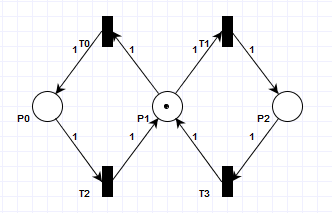
\includegraphics[width=\textwidth]{image1.png}
 % \caption{}
\end{figure}

The states are as follows:
\begin{itemize}
 \item S1(1,0,0)
 \item S2(0,1,0)
 \item S3(0,0,1)
\end{itemize}

Net 1 can run infinitely, because it does not have a deadlock, all the states
are vanishing, and in all the states there is an enabled transition.\\

\textit{Modify the network to the below setting, and again generate all possible states. Explain why these states are different from states generated above (use proper terminology, such as predicates, places, tokens, firing, and transitions). Can this network run infinitely long, and if not what are the end-states?
 Note that arcs have numbers on them, and there is a different initial marking.
}

\begin{figure}[H]
 \centering
 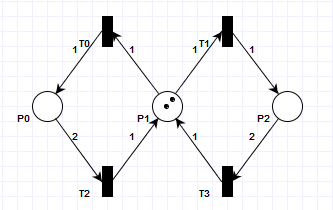
\includegraphics[width=\textwidth]{image2.png}
 % \caption{}
\end{figure}

The states are as follows:
\begin{itemize}
 \item S0(0,2,0)
 \item S1(0,1,1)
 \item S2(1,1,0)
 \item S3(0,0,2)
 \item S4(1,0,1)
 \item S5(2,0,0)
 \item S6(0,1,0)
 \item S7(0,0,1)
 \item S8(1,0,0)
\end{itemize}

The states are different from the states generated above, because the initial
marking is different, the initial marking is now (0,2,0), and the weight for arcs
on transitions T2 and T3 are changed, so the possible firing sequences are also
different.

This network cannot run infinitely long, because there is deadlocks in the network.
The end states are S4, S7, S8 which are all deadlock situations.



\section{}

\textit{Build a semaphore network with the below initial marking, as shown below. Process 1 is denoted on the left, and process 2 on the right.
}
\begin{figure}[H]
 \centering
 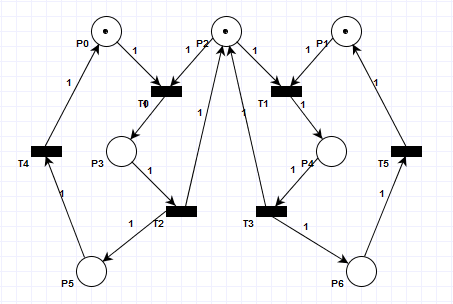
\includegraphics[width=\textwidth]{image3.png}
 % \caption{}
\end{figure}

\textit{Answer the following questions:}

\subsection{}
\textit{Enumerate all states of the semaphore in the (P0, P1, P2, P3, P4, P5, P6) format.Hint: you can use "Analysis Module Manager $\rightarrow$ Reachability/Coverability Graph" option.
}
\\
\\S0: (1, 1, 1, 0, 0, 0, 0)
\\S1: (1, 0, 0, 0, 1, 0, 0)
\\S2: (0, 1, 0, 1, 0, 0, 0)
\\S3: (1, 0, 1, 0, 0, 0, 1)
\\S4: (0, 1, 1, 0, 0, 1, 0)
\\S5: (0, 0, 0, 1, 0, 0, 1)
\\S6: (0, 0, 0, 0, 1, 1, 0)
\\S7: (0, 0, 1, 0, 0, 1, 1)

\subsection{}
\textit{Which of the states represent a situation when process 1 OR process 2 take possession of the shared resource?}\\ \\
S1, S2, S5, S6

\subsection{}
\textit{Is it possible to reach state (0, 0, 0, 1, 1, 0, 0)? What does this state represent?}
\\
\\This state represents a token in P3 and a token in P4. It is not possible because the state is not found inside the reachability/coverability graph. (The resource is shared.)

\section{}

\begin{figure}[H]
 \centering
 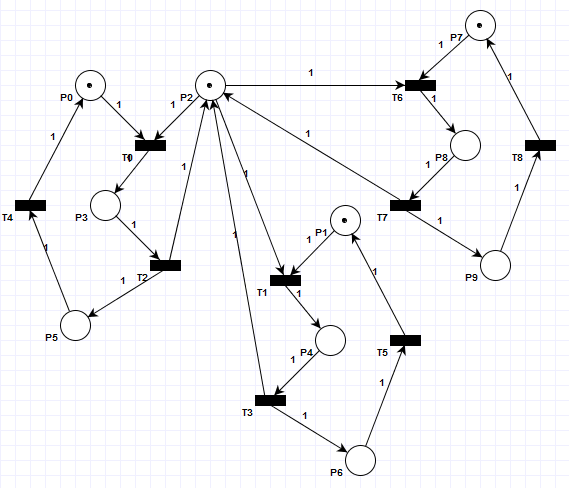
\includegraphics[width=\textwidth]{image4.png}
 % \caption{}
\end{figure}

\textit{Answer the following questions:}

\subsection{}
\textit{How many states does this network have?
}\\

This network has 20 states (S0 - S19).

\subsection{}
\textit{Which places are responsible for showing if a given process has access to the shared resource?}

P2 holds the shared resource.

For the process on the left, P3 is responsible for showing the process has access
to the shared resource, because when P3 holds a token, the shared token originally
located at P2 is used by the left side process.

For the process on the bottom, P4 is responsible for showing the process has access
to the shared resource, because when P4 holds a token, the shared token originally
located at P2 is used by the bottom side process.

For the process on the right, P8 is responsible for showing the process has access
to the shared resource, because when P8 holds a token, the shared token originally
located at P2 is used by the right side process.

\subsection{}
\textit{Is it possible that this network will have more than 4 OR less than 3 tokens in any possible state?
 If yes, then list these states.
}\\

No, this is not possible because the minimum is 3 and the maximum is 4.

\subsection{}
\textit{Generate four starvation cycles for this network. Represent the cycles in terms of the firing sequences. Is it possible to have more than 4 starvation cycles for this network?}\\


$<$T0, T2, T4, T0, T2...$>$\\

$<$T1, T3, T5, T1, T3...$>$\\

$<$T6, T7, T8, T6, T7...$>$\\

$<$T0, T2, T1, T3, T5, T4, T0, T2...$>$\\

More than 4 starvation cycles are possible.
This depends on the firing priorities.




\subsection{}
\textit{Modify the 3 processes semaphore model to the below one, including the initial marking.
 Note that some arcs have numbers on them, and there is a different initial marking.
}

\begin{figure}[H]
 \centering
 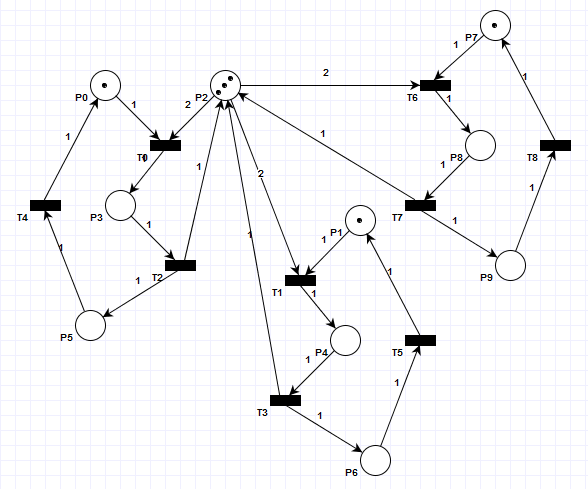
\includegraphics[width=\textwidth]{image5.png}
 % \caption{}
\end{figure}

\textit{Is it possible that two processes will be able to access the shared resource at the same time in the above model? If yes, then give the state that shows this situation.}\\

% NOTE check this!!!
% Yes, two processes will be able to access the shared resource at the same time.\\
% One such state is ()\\

No, this is not possible. The processes can run at the same time,
but they won't be able to access the shared resource simultaneously.\\

\textit{Is the number of tokens bounded in this network (is it possible to have a place that may have continuously increasing number of tokens)? If yes, then what is the maximum number of tokens in the network? Also, in this case list all the states in which the maximum number of tokens occurs.
 Use the (P0, P1, P2, P3, P4, P5, P6, P7, P8, P9) format
}\\

\noindent The network is bounded\\
the maximum number of tokens is 6\\
it occurs in state:\\
S0(1, 1 ,3 ,0 ,0 ,0 ,0 ,1 ,0 ,0)

\textit{What is the minimum number of tokens in the above network?}\\

the minimum number of tokens in the above network is 3

\section{}

\textit{Start by loading and compiling the two semaphores network model created in TASK 2. Use the “Analysis module manager” section.}

\subsection{}
\textit{Perform the state enumeration with initial marking (1, 1, 1, 0, 0, 0, 0), and answer the following questions}

The states are as follows:
\begin{itemize}
 \item S0(1, 1, 1, 0, 0, 0, 0)
 \item S1(1, 0, 0, 0, 1, 0, 0)
 \item S2(0, 1, 0, 1, 0, 0, 0)
 \item S3(1, 0, 1, 0, 0, 0, 1)
 \item S4(0, 1, 1, 0, 0, 1, 0)
 \item S5(0, 0, 0, 1, 0, 0, 1)
 \item S6(0, 0, 0, 0, 1, 1, 0)
 \item S7(0, 0, 1, 0, 0, 1, 1)
\end{itemize}

\subsubsection{}
\textit{How many reachable states are there for this network and initial marking?}\\

There are eight reachable states for this network and initial marking.

\subsubsection{}
\textit{How many places in this network never receive any tokens, how many receive a single token, and how many receive more than one token}\\

\noindent no tokens: 0 places -- None\\
single token: 7 places -- P0, P1, P2, P3, P4, P5, P6\\
more than one token: 0 places -- None\\

\subsubsection{}
\textit{Explain what does it mean that a network is strictly conservative}\\

It means that the total number of tokens in the Petri Net is constant.

\subsubsection{}
\textit{Does the network have any deadlocks, is it bounded and safe?}\\

The network does not have any dealocks, it is bounded and safe.

\subsubsection{}
\textit{List all t-invariants of the network.}\\ \\
T-Invariants: \\
format: (T0 T1 T2 T3 T4 T5) \\

\noindent (0 1 0 1 0 1) \\
(1 0 1 0 1 0) \\

\subsection{}
\textit{Perform the state enumeration with initial marking (2, 0, 2, 0, 0, 0, 0), and answer the following questions.}\\

The states are as follows:
\begin{itemize}
 \item S0(2, 0, 2, 0, 0, 0, 0)
 \item S1(1, 0, 1, 1, 0, 0, 0)
 \item S2(1, 0, 2, 0, 0, 1, 0)
 \item S3(0, 0, 0, 2, 0, 0, 0)
 \item S4(0, 0, 1, 1, 0, 1, 0)
 \item S5(0, 0, 2, 0, 0, 2, 0)
\end{itemize}

\subsubsection{}
\textit{Which transitions can be fired in state S2 (1, 0, 2, 0, 0, 1, 0)?}\\

T0, T4

\subsubsection{}
\textit{List all the reachable states in the (P0, P1, P2, P3, P4, P5, P6) format}\\

The reachable states are as follows:
\begin{itemize}
 \item S0(2, 0, 2, 0, 0, 0, 0)
 \item S1(1, 0, 1, 1, 0, 0, 0)
 \item S2(1, 0, 2, 0, 0, 1, 0)
 \item S3(0, 0, 0, 2, 0, 0, 0)
 \item S4(0, 0, 1, 1, 0, 1, 0)
 \item S5(0, 0, 2, 0, 0, 2, 0)
\end{itemize}

\subsubsection{}
\textit{How many places in this network never receive any tokens, how many receive a single token, and how many receive more than one token}\\
\noindent\\
no tokens: 3 states -- P1, P4, P6\\
single token: -- None\\
more than one token: 4 states -- P0, P2, P3, P5\\


\section{}

Screenshots of the lab VM for each of the group members:

\begin{figure}[H]
 \centering
 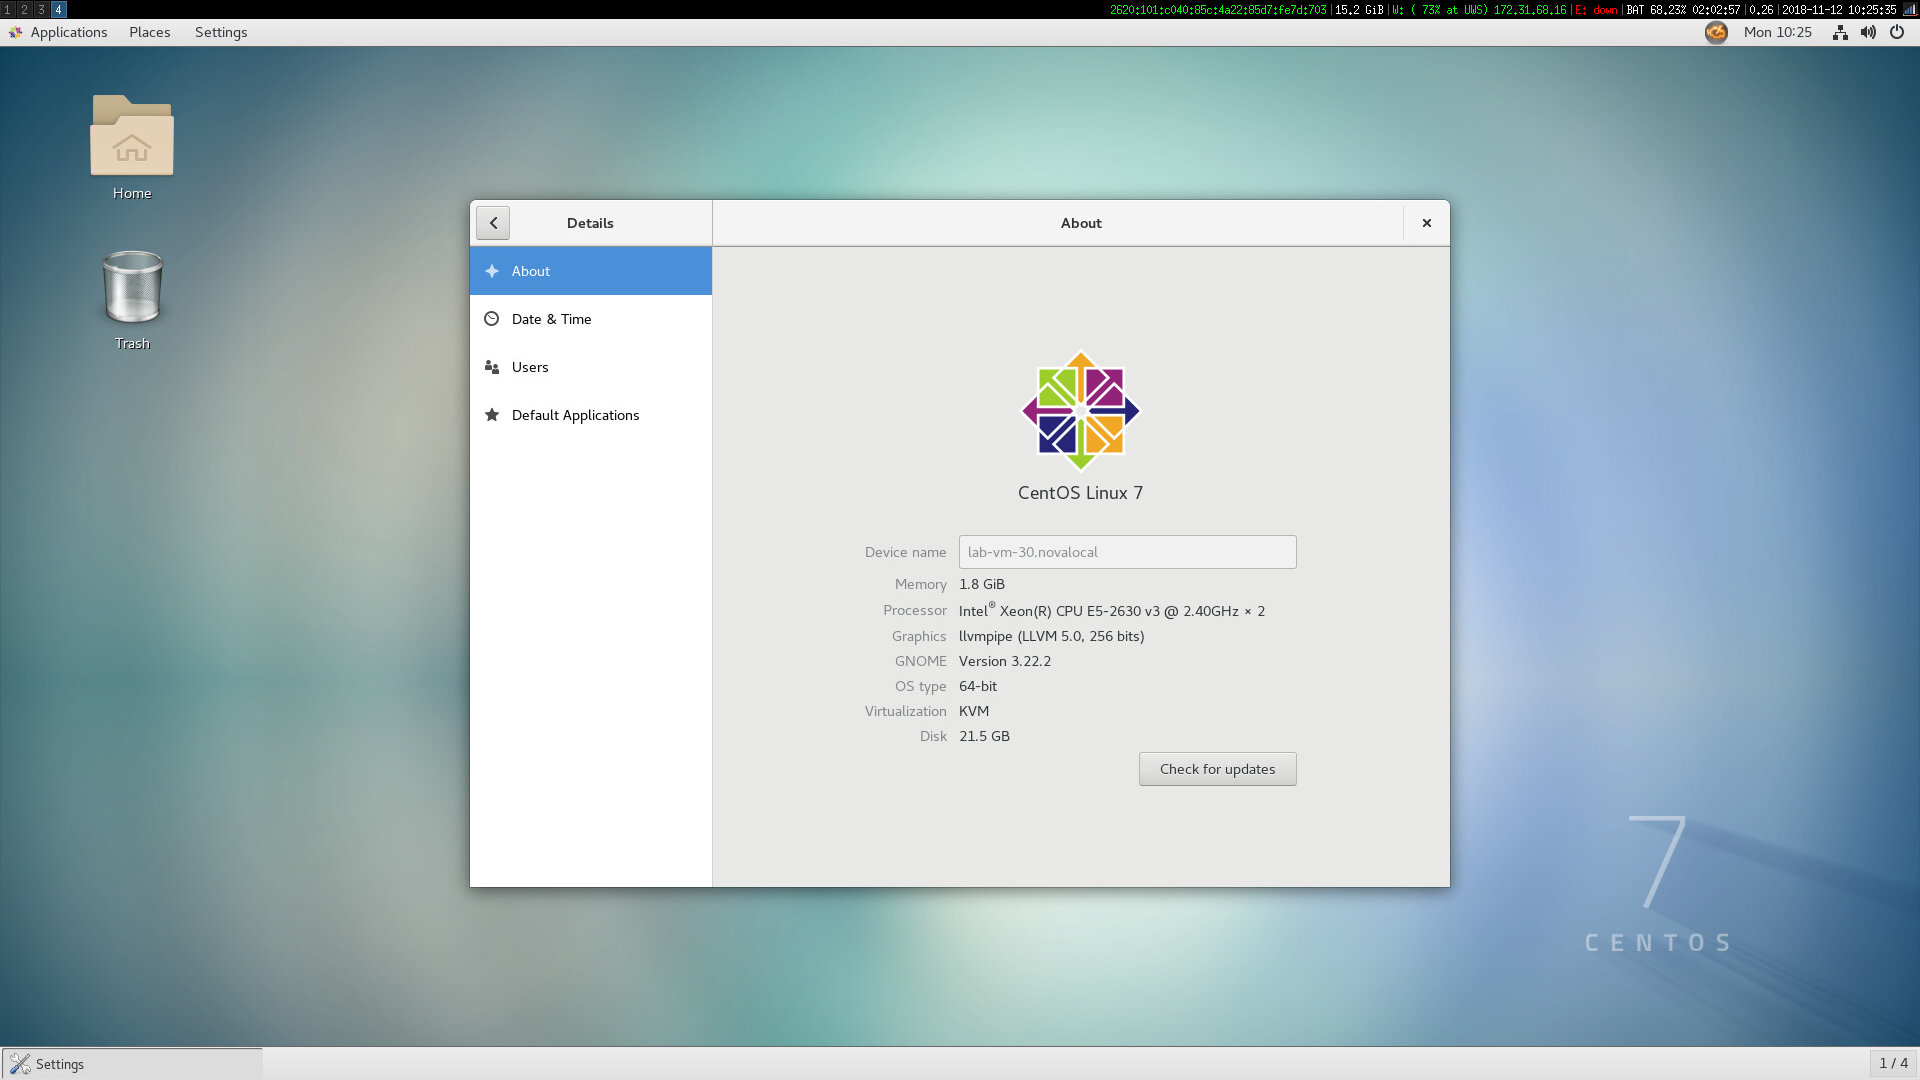
\includegraphics[width=\textwidth]{arun.png}
 \caption{Arun Woosaree}
\end{figure}

\begin{figure}[H]
 \centering
 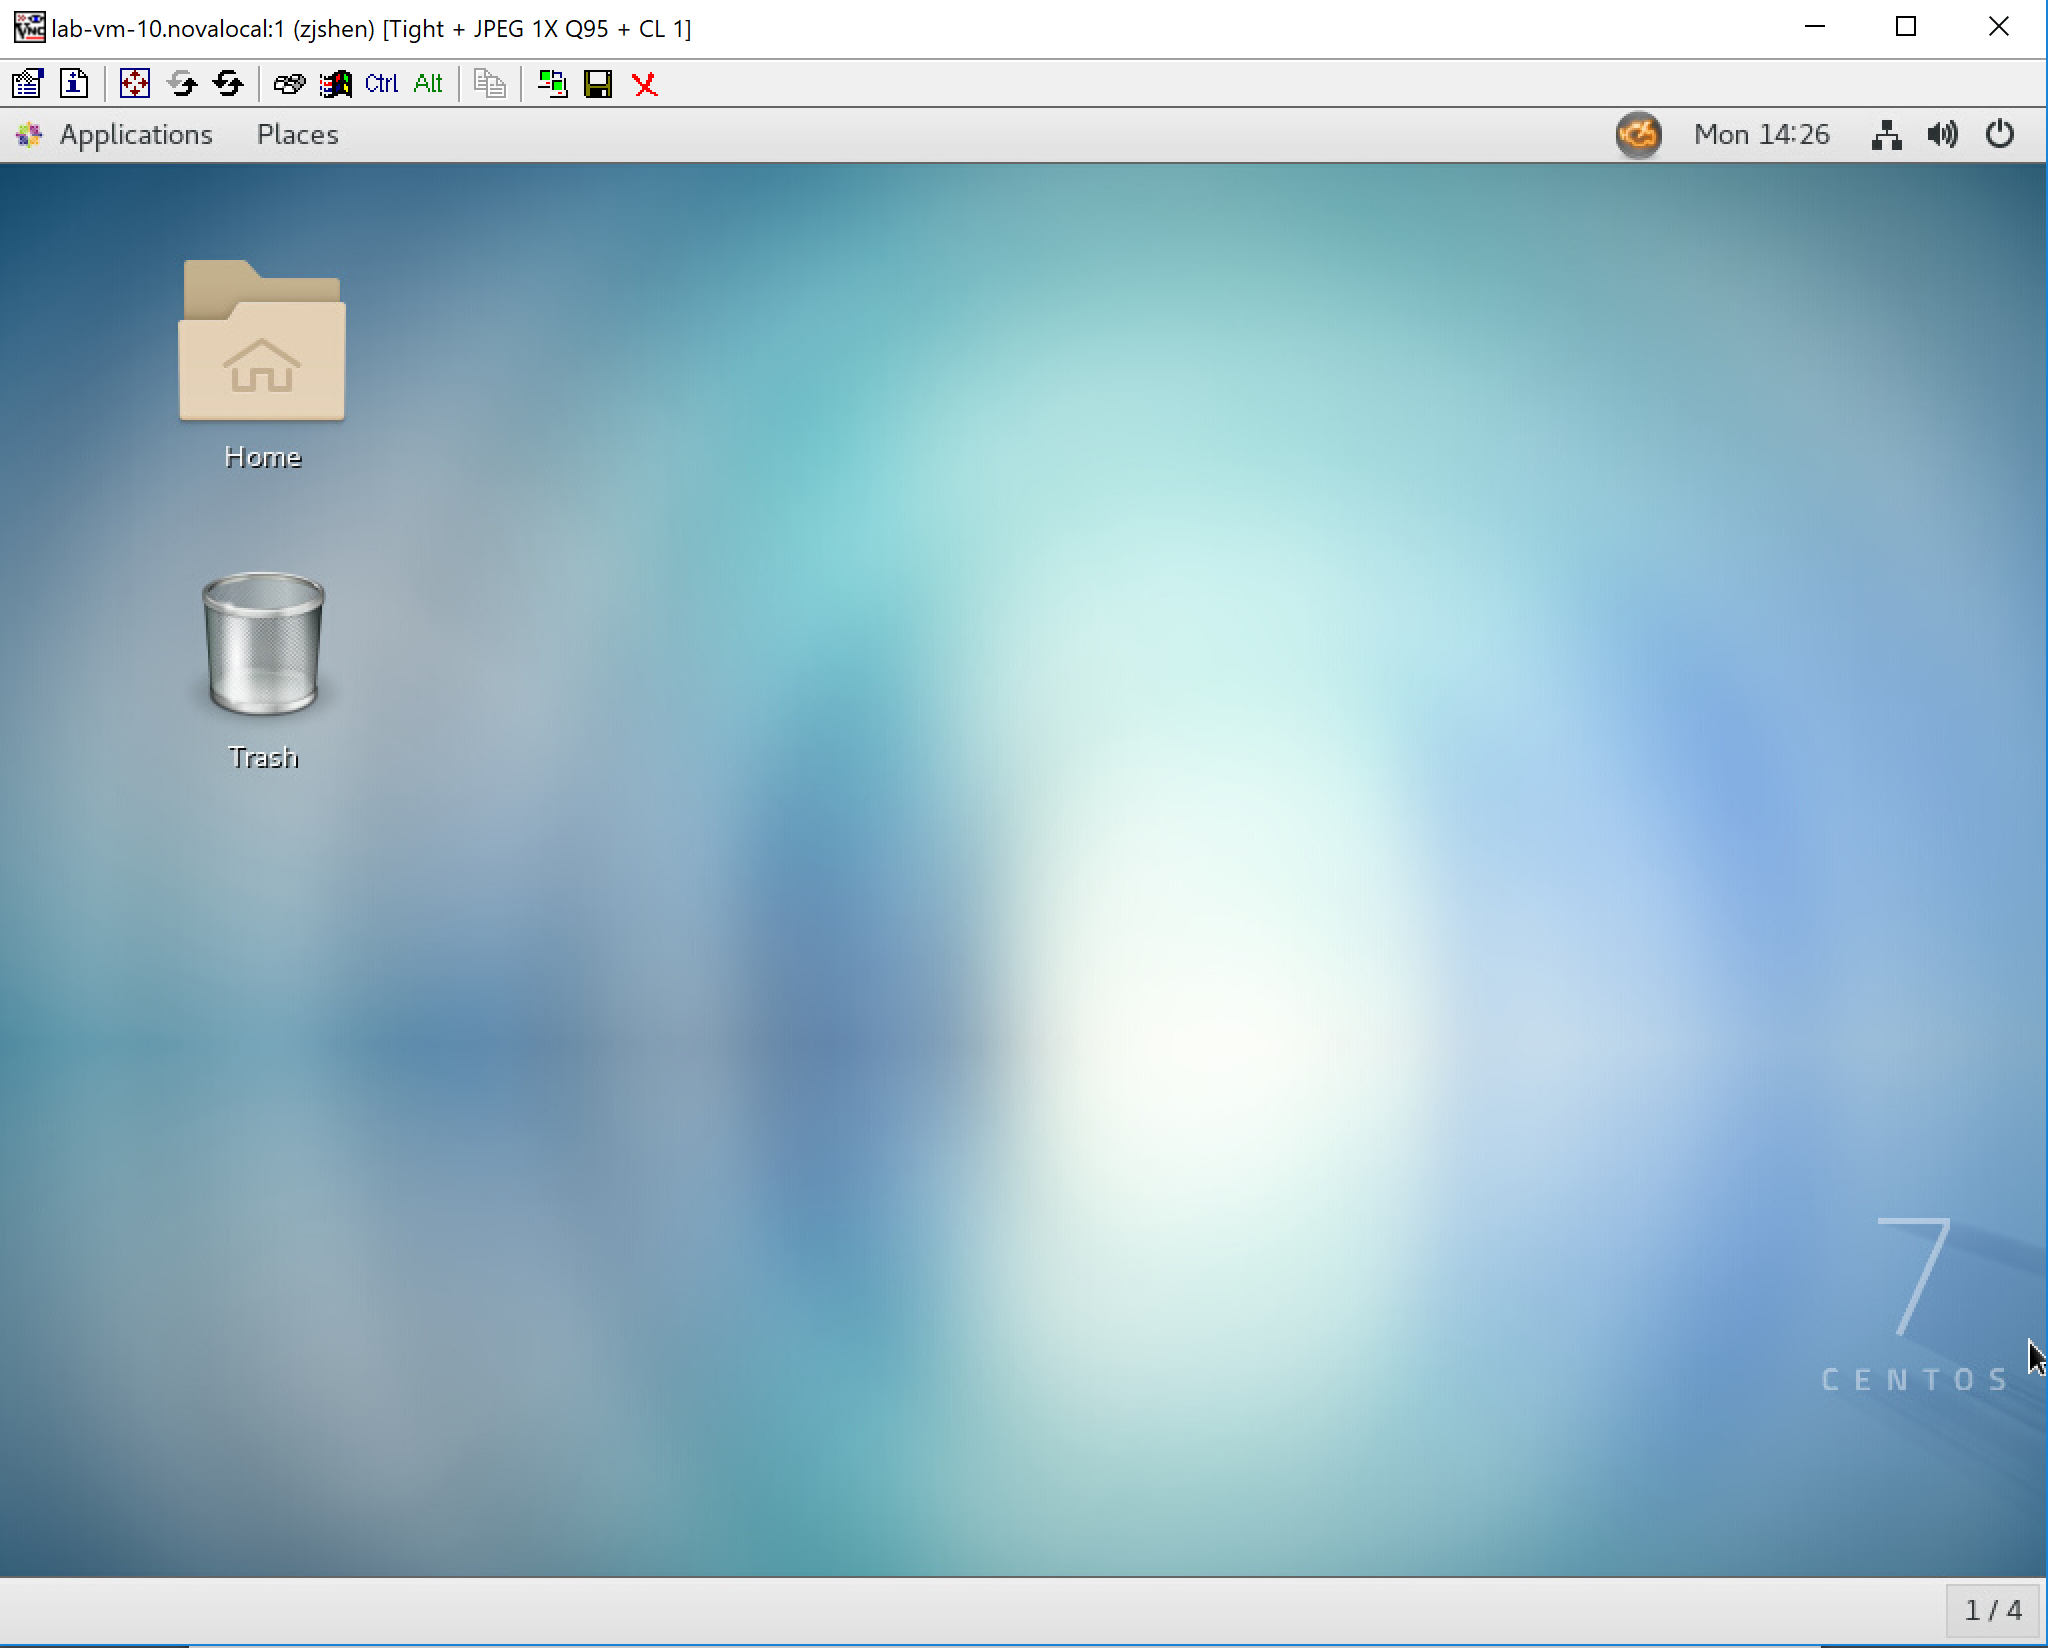
\includegraphics[width=\textwidth]{max.PNG}
 \caption{Zhi Shen}
\end{figure}

\begin{figure}[H]
 \centering
 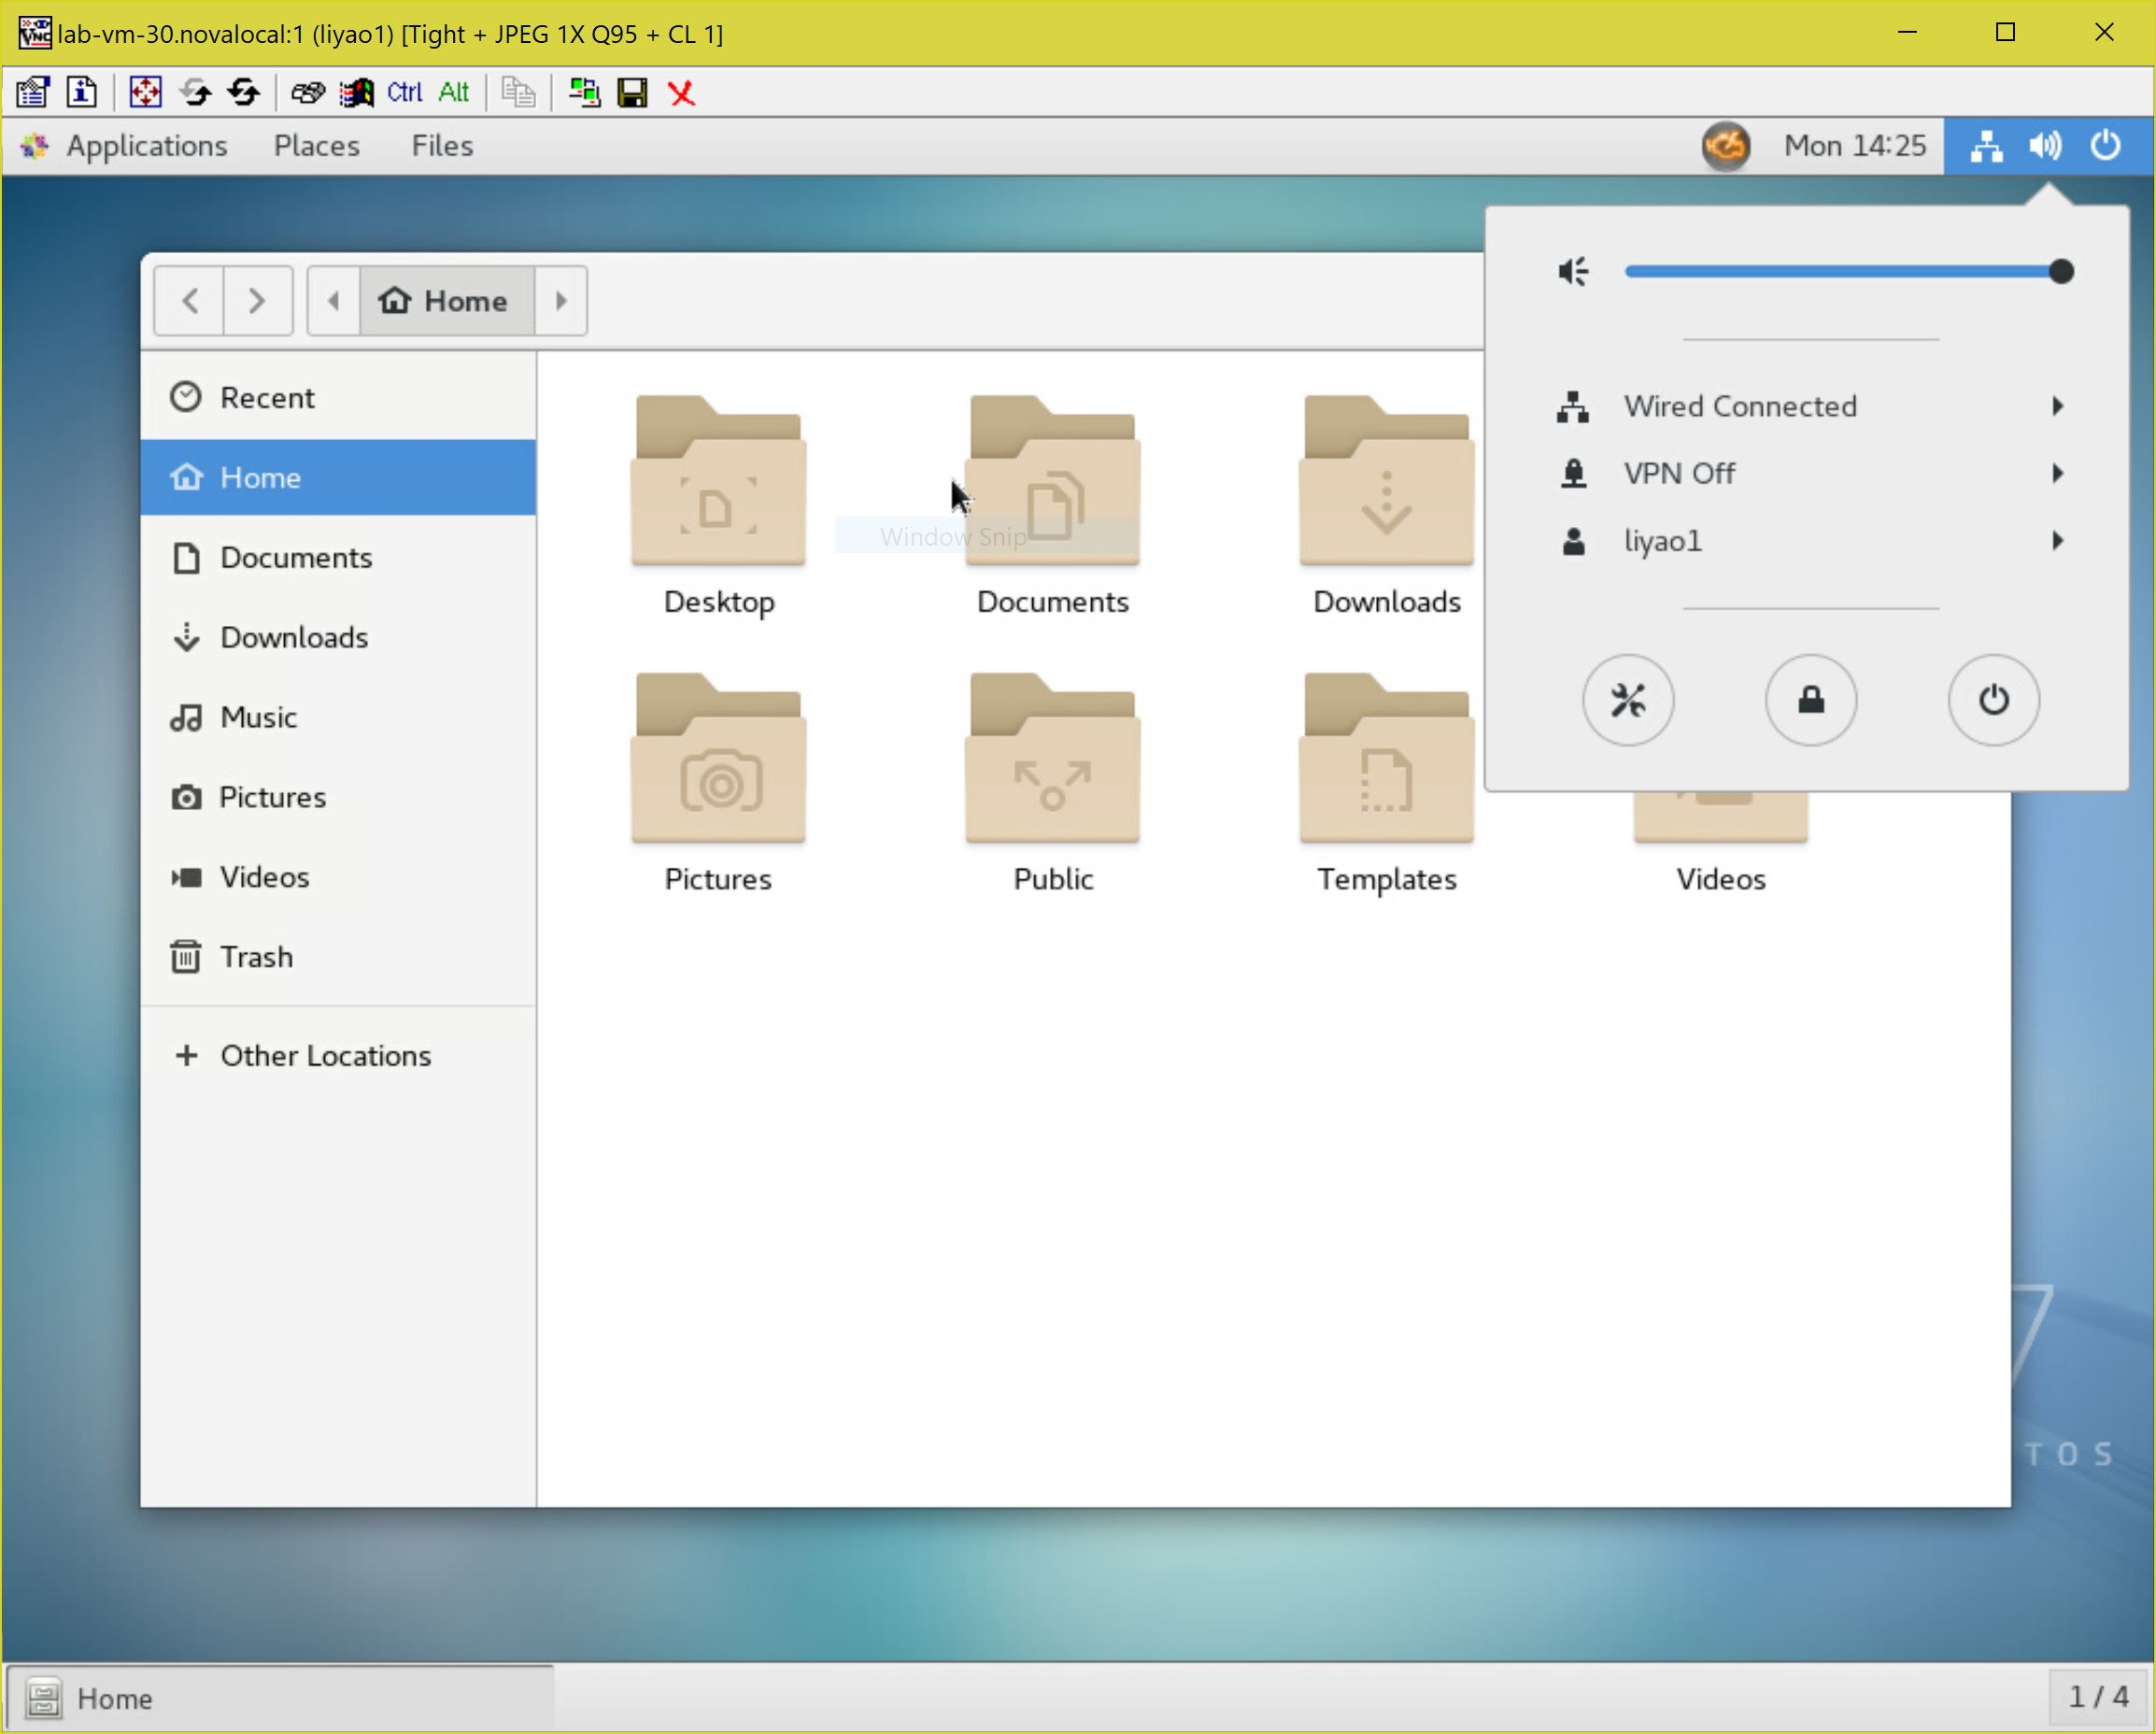
\includegraphics[width=\textwidth]{liyao.JPG}
 \caption{Liyao Jiang}
\end{figure}

\end{document}
